\documentclass[border=6pt]{standalone}
\usepackage{tikz}
\usetikzlibrary{arrows.meta,calc}
\begin{document}
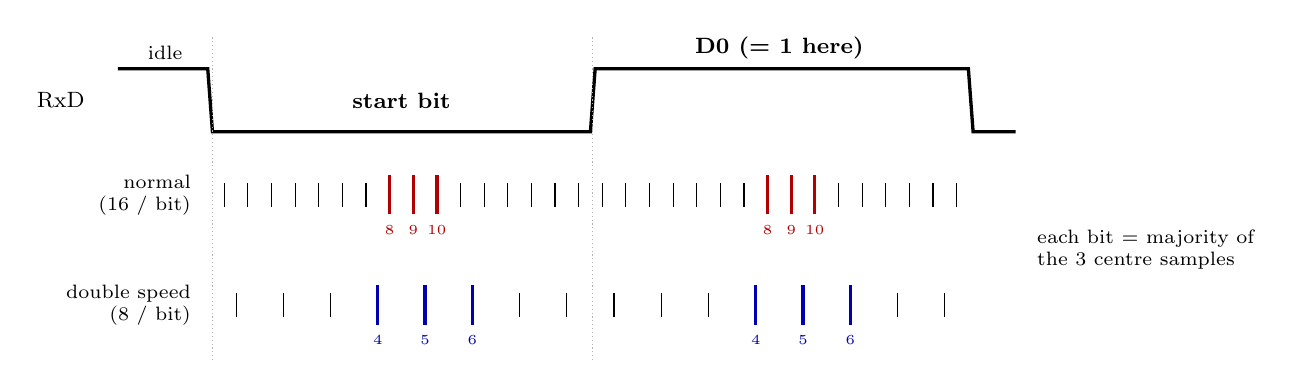
\begin{tikzpicture}[>=Stealth,font=\small,x=0.3cm,y=1cm]
% one bit = 16 units; start bit from 0 to 16, D0 from 16 to 32
\def\h{0.8}
\node[anchor=east,font=\footnotesize] at (-5,0.4) {RxD};
\draw[very thick] (-4,\h) -- (-0.2,\h) -- (0,0) -- (16,0) -- (16.2,\h) -- (32,\h) -- (32.2,0) -- (34,0);
\node[font=\footnotesize\bfseries] at (8,0.4) {start bit};
\node[font=\footnotesize\bfseries,anchor=south] at (24,\h) {D0 (= 1 here)};
\node[font=\scriptsize,anchor=south] at (-2,\h) {idle};
\draw[gray!60,densely dotted] (16.1,-2.9) -- (16.1,1.2);
\draw[gray!60,densely dotted] (0,-2.9) -- (0,1.2);
% normal: 16 samples per bit
\node[anchor=east,font=\scriptsize,align=right] at (-0.5,-0.8) {normal\\(16 / bit)};
\foreach \b in {0,16} \foreach \k in {1,...,16} {
  \pgfmathsetmacro{\x}{\b+\k-0.5}
  \pgfmathtruncatemacro{\v}{(\k>7)*(\k<11)}
  \ifnum\v=1 \draw[red!70!black,very thick] (\x,-1.05) -- (\x,-0.55); \else \draw (\x,-0.95) -- (\x,-0.65); \fi
}
\foreach \b in {0,16} \foreach \k in {8,9,10} \node[font=\tiny,red!70!black] at (\b+\k-0.5,-1.25) {\k};
% double speed: 8 samples per bit
\node[anchor=east,font=\scriptsize,align=right] at (-0.5,-2.2) {double speed\\(8 / bit)};
\foreach \b in {0,16} \foreach \k in {1,...,8} {
  \pgfmathsetmacro{\x}{\b+2*\k-1}
  \pgfmathtruncatemacro{\v}{(\k>3)*(\k<7)}
  \ifnum\v=1 \draw[blue!70!black,very thick] (\x,-2.45) -- (\x,-1.95); \else \draw (\x,-2.35) -- (\x,-2.05); \fi
}
\foreach \b in {0,16} \foreach \k in {4,5,6} \node[font=\tiny,blue!70!black] at (\b+2*\k-1,-2.65) {\k};
\node[font=\scriptsize,align=left,anchor=west] at (34.5,-1.5) {each bit = majority of\\the 3 centre samples};
\end{tikzpicture}
\end{document}
